%% MAC-IRL — ICAIF '26 submission
%% Template: acmart sigconf + anonymous (required by ICAIF '26 CFP)
%% Compile: pdflatex -> bibtex -> pdflatex -> pdflatex   (or use Overleaf)
%% HARD LIMIT: 8 pages total, including all figures and references.
%% Double-blind: no author names/affiliations; cite own work in third person.
%%
%% STATUS (2026-08-02)
%%   Sections 1-5: full draft in this file (§1-§3 merged with §4-§5 on 2026-07-31)
%%   Numbers    : canonical run = runs/continuous_reward3_lambda_unified/  (lambda unified at 0.005)
%%   Validation : runs/continuous_reward3_lambda_validation/
%%   References : verified 2026-07-24, see docs/refs_checklist.md
%%   Checklist  : docs/paper_checklist.md

\documentclass[sigconf,anonymous,review]{acmart}

%% Figure 1 (the Section 3 pipeline) is drawn in TikZ so that its symbols
%% are typeset in the body font rather than baked into a bitmap.
\usepackage{tikz}
\usetikzlibrary{arrows.meta,positioning,fit,backgrounds,calc}

%% 4-5장 그림 자리. 이미지 파일(fig_*.pdf/png)이 있으면 그것을 쓰고,
%% 없으면 같은 높이의 안내 박스를 그려 페이지 수가 실제와 어긋나지 않게 한다.
\newcommand{\figorbox}[2]{%
  \IfFileExists{#1.pdf}{\includegraphics[width=\linewidth]{#1.pdf}}{%
  \IfFileExists{#1.png}{\includegraphics[width=\linewidth]{#1.png}}{%
    \fbox{\parbox[c][#2][c]{\dimexpr\linewidth-2\fboxsep-2\fboxrule\relax}%
      {\centering\ttfamily\footnotesize figure file not found:\\ \detokenize{#1}.pdf / \detokenize{#1}.png}}}}}


\AtBeginDocument{%
  \providecommand\BibTeX{{Bib\TeX}}}

%% Rights: placeholder values until the rights form is completed.
\setcopyright{acmlicensed}
\copyrightyear{2026}
\acmYear{2026}
\acmDOI{XXXXXXX.XXXXXXX}
\acmConference[ICAIF '26]{7th ACM International Conference on AI in
  Finance}{November 14--17, 2026}{Milan, Italy}
\acmISBN{978-1-4503-XXXX-X/2026/11}

\begin{document}

%% The optional argument is the RUNNING HEAD. Without it acmart puts the
%% full title in the header on odd pages, where it collides with the
%% conference line. Added 2026-07-28.
\title[Same Signals, Different Actions]{Same Signals, Different Actions:
  Recovering and Validating
  Investor-Type Preferences from Daily Flow via Inverse Reinforcement
  Learning}

%% NOTE: ICAIF '26 review is DOUBLE-BLIND. The "anonymous" class option
%% suppresses the author block below in the compiled PDF, so the
%% submission stays anonymous while the information is retained here for
%% the camera-ready version. Remove "anonymous" only after acceptance.
\author{Yonghwa Shin}
\affiliation{%
  \institution{Soongsil University}
  \city{Seoul}
  \country{Republic of Korea}}
\email{andysheen607@gmail.com}

\author{Yumin Kwon}
\affiliation{%
  \institution{Soongsil University}
  \city{Seoul}
  \country{Republic of Korea}}

\begin{abstract}
Foreign, institutional, and retail investors trade the same asset for
different reasons, yet the regularities that describe them have been
established one phenomenon at a time, leaving no common scale on which
their preferences can be compared. We build such a scale with inverse
reinforcement learning: each type is an agent whose daily net-buy
intensity reveals a latent reward over shared market-state features, and
all three are estimated under one shared specification, so that
differences come only from what is learned. Under a one-step horizon this
estimator coincides with a Lasso; our contribution is therefore a
validation protocol rather than a new estimator---out-of-sample stability
under purged cross-validation and a block bootstrap, construct-validity
checks against established behavioral regularities, and explicit
disclosure of null results. On 973 trading days of Samsung Electronics
(005930) flow, we find that foreign and retail flow load with opposite
signs on momentum, each sign-consistent across all 45 out-of-sample
splits, while institutional flow reveals no distinct tendency. Applied
unchanged to a second stock, Hyundai Motor (005380), the foreign and
retail direction partly persists while institutional flow again stays
near chance.
\end{abstract}

\begin{CCSXML}
<ccs2012>
 <concept>
  <concept_id>10010147.10010257.10010293.10010294</concept_id>
  <concept_desc>Computing methodologies~Inverse reinforcement learning</concept_desc>
  <concept_significance>500</concept_significance>
 </concept>
 <concept>
  <concept_id>10002944.10011122.10002945</concept_id>
  <concept_desc>General and reference~Validation</concept_desc>
  <concept_significance>300</concept_significance>
 </concept>
 <concept>
  <concept_id>10010405.10010481.10010485</concept_id>
  <concept_desc>Applied computing~Economics</concept_desc>
  <concept_significance>300</concept_significance>
 </concept>
</ccs2012>
\end{CCSXML}

\ccsdesc[500]{Computing methodologies~Inverse reinforcement learning}
\ccsdesc[300]{General and reference~Validation}
\ccsdesc[300]{Applied computing~Economics}

\keywords{Inverse reinforcement learning, investor behavior, order flow,
  behavioral finance, interpretability, model validation}

\maketitle

\section{Introduction}

On the same day, in the same stock, and facing the same public
information, investors act differently. Which conditions tilt each
investor type toward buying or toward selling? This is a basic question
for price formation, for market microstructure, and for
investor-protection policy, since type-level flow is where behavioral
tendencies reach the market. The problem we address is how to
recover, from observed daily flow alone, a description of what each
investor type responds to---and to recover it in a form that can be
compared across types.

Existing evidence does not deliver that comparison. The stylized
regularities of type-specific behavior---momentum versus contrarian
trading~\cite{grinblatt_keloharju2001}, the disposition
effect~\cite{shefrin_statman,odean1998}, institutional
herding~\cite{lakonishok_shleifer_vishny}---have been established one
phenomenon at a time, in separate reduced-form regressions on different
samples and specifications; of the third we operationalize only the
own-following component~\cite{sias2004}, for the reason given in
Section~\ref{sec:method-features}. Asset demand systems~\cite{koijen_yogo2019}
do estimate type-level preferences within a single framework, but from
quarterly holdings rather than daily flow, and without behavioral state
variables. As a result, even a simple comparison---does foreign flow load
more strongly on momentum than retail flow does?---has not been answered
under a shared specification.

We approach this problem through inverse reinforcement
learning~\cite{ziebart2008}. Each investor type is treated as an agent
whose observed daily net-buy intensity reveals a latent reward defined
over interpretable market-state features. A concave reward makes the
optimal action graded, so trading intensity is derived rather than
assumed. The three types are estimated under one \emph{shared
specification}, with only the parameters learned separately from each
type's own data---so that any difference between types reflects what is learned
rather than what was designed, and the estimated coefficients lie on a
common scale. In this
myopic formulation, the estimator coincides exactly with a
Lasso~(\S\ref{sec:method}). We state this rather than obscure it, and
build interpretation and validation on top of it: the recovered rewards
are checked for out-of-sample stability under combinatorial purged
cross-validation~\cite{lopezdeprado2018}, for agreement with
independently established behavioral regularities, and for what they
fail to identify.

Our contributions are as follows.

\begin{itemize}
  \item \textbf{A shared-specification design that places investor types
    on a common scale.} Where prior evidence is single-phenomenon or
    quarterly, estimating all three types identically from daily flow
    makes their weights comparable \emph{in magnitude, not only in sign},
    so that regularities established separately can be read against one
    another within a single fit.
  \item \textbf{A validation protocol for which recovered weights to
    trust.} A coefficient is interpreted only when its sign is stable
    across resampling and re-estimation \emph{and} its bootstrap interval
    excludes zero; surviving signs are checked against independently
    established behavioral regularities, and everything that fails the
    rule---including converged but unidentified coefficients---is reported
    as a null rather than interpreted.
  \item \textbf{Empirical results on daily Korean flow.} On 973 trading
    days of Samsung Electronics, foreign and retail flow oppose each other
    on momentum while sharing positive persistence in their own flow, and
    institutional flow shows no distinct tendency. Applied without
    refitting to a second stock (Hyundai Motor), the foreign and retail
    direction partly persists---a partial regularity, not a
    stock-invariant law.
\end{itemize}

On a common scale, these results locate the difference between types
precisely: they differ not in whether their flow persists but in the
direction they continue, and at the aggregate level the institutional
category yields no comparable signal of its own.

The remainder of the paper is organized as follows. Section~2 reviews
related work; Section~3 presents the model together with the estimation
and validation methodology; Section~4 reports experiments and results;
and Section~5 discusses implications, limitations, and future work,
including the extension to structural reward recovery.

\section{Related Work}
\label{sec:related}

To place our contribution, we review four lines of work and note what
each leaves open.

\textbf{Empirical evidence on investor-type flows.} That trading behavior
differs systematically across investor types is well documented across
markets~\cite{choe_kho_stulz,grinblatt_keloharju2001,kaniel_saar_titman}.
Korean foreign flow shows positive-feedback trading and daily
herding~\cite{choe_kho_stulz}, and short-horizon contrarian patterns
appear in US individual flow~\cite{kaniel_saar_titman}. The sharpest
evidence comes from a Finnish register recording every investor's daily
buys, sells, and holds: Grinblatt and
Keloharju~\cite{grinblatt_keloharju2001} find contrarian behavior
strongest among households, while foreign investors tend to be momentum
traders. The topic remains active---Oh~\cite{oh2025} applies detrended
fluctuation analysis to Korean daily flows from 2015 to 2024 and finds
long-range dependence in all three types, with the cross-type ranking
visible in gross buys and sells attenuating once flows are netted. These findings, however, either characterize the
time-series properties of flow or come from separate regressions on
different samples and specifications, each targeting one phenomenon at a
time, so the resulting coefficients cannot be placed side by side across
types.

\textbf{Behavioral regularities behind type differences.} Three
regularities recur across this literature. Medium-term return
persistence underlies momentum and contrarian
trading~\cite{jegadeesh_titman}. The disposition effect---reluctance to
realize losses~\cite{shefrin_statman,odean1998}---is documented in US
brokerage accounts and recovered from daily Finnish
trades~\cite{grinblatt_keloharju2001}. Herding
measures~\cite{lakonishok_shleifer_vishny} capture participants
\emph{of the same type} trading a stock simultaneously;
Sias~\cite{sias2004} separates institutions that follow each other from
institutions that follow their own lagged trades. Each regularity has
been established in isolation, for one phenomenon and often one investor
type, so none of them indicates how strongly a given type weighs one
regularity against another.

\textbf{Demand systems for heterogeneous investors.} A separate line
estimates type-level preferences within a single framework. Koijen and
Yogo~\cite{koijen_yogo2019} develop a characteristics-based demand system
and estimate it on Form 13F holdings, recovering how demand varies across
institution types and what that heterogeneity implies for prices. The
estimation applies a shared specification to all investors, as we
require, but
it operates on \emph{quarterly} holdings and on firm fundamentals rather
than the behavioral state variables where the regularities above are
defined. Daily flow falls outside its scope.

\textbf{Inverse reinforcement learning and preference estimation in
finance.} Inverse reinforcement learning recovers a reward that
rationalizes observed behavior, with non-uniqueness resolved by the
maximum-entropy principle~\cite{ziebart2008}. In finance the dominant use is
learning or improving trading strategies: a sentiment-based reward
learned with Gaussian process IRL to drive a trading
system~\cite{yang2018gpirl}, strategy recovery under transaction
costs~\cite{sun2023transaction}, and---closest to our setting---Halperin
et al.~\cite{halperin2022}, who recover the implied reward of individual
fund managers and feed it to a forward RL algorithm to improve their
allocations. Outside finance the same machinery has been used to
interpret behavior rather than to trade, for instance to characterize
risk-prone and risk-averse decision making~\cite{liu2019risk}. The shared objective in this line is a profitable policy or
the reward of a single actor, recovered to be imitated or improved. To our knowledge, no prior work estimates the rewards of
\emph{heterogeneous investor types} on a shared feature set so that they
can be compared with one another, nor subjects the recovered rewards
themselves to out-of-sample stability and construct-validity testing.

\section{Method}
\label{sec:method}

%% are typeset in the body font. Kept in sync with the text: three state
%% features (momentum, flow persistence, loss region), two contexts, one
%% shared specification, five validation procedures. The output box names
%% the deliverable; fitted values belong to Section 4.
%%
%% Layout notes, so the boxes stay collision-free if edited:
%%  - every stage has the same minimum height, so the tallest content
%%    (Validation: title + 2x2 grid + ablation row) sets the box height
%%    and nothing spills over a border;
%%  - inner cells are placed from the stage's NORTH anchor, not its
%%    centre, so adding a line to one stage does not move another's cells;
%%  - the two context cells are pushed left and right of centre to leave
%%    a clear vertical channel for the dashed feedback arrow;
%%  - \resizebox absorbs the last few percent of width, so the scale
%%    factor stays close to one and the type near body size.
%% =====================================================================
\begin{figure*}[t]
\centering
\resizebox{\textwidth}{!}{%
\begin{tikzpicture}[
  font=\scriptsize,
  >={Stealth[length=4pt]},
  stage/.style={draw, rounded corners=1.5pt, align=center, inner sep=2.5pt,
                minimum height=27mm, text width=#1, anchor=west},
  cell/.style={draw, rounded corners=1pt, fill=black!5, align=center,
               inner sep=1.5pt, font=\tiny, text width=#1},
  ctx/.style={cell=#1, fill=black!14},
  hdr/.style={anchor=north, font=\scriptsize\bfseries, align=center, inner sep=0pt},
  lbl/.style={font=\tiny\itshape, inner sep=1pt},
  flow/.style={->, semithick},
  gap/.store in=\gap, gap=5mm,
]

%% ---- 1 input --------------------------------------------------------
\node[stage=18mm] (inp) at (0,0) {};
\node[hdr] (inph) at ([yshift=-2.5mm]inp.north) {Input};
\node[anchor=north, align=center, text width=17mm, font=\tiny]
  at ([yshift=-1.5mm]inph.south)
  {investor type $i$,\\ trading day $t$\\[3pt]
   observed action\\ $u_{i,t}$\\[3pt]
   target $a_{i,t+1}$};

%% ---- 2 state features and context -----------------------------------
\node[stage=46mm] (feat) at ([xshift=\gap]inp.east) {};
\node[hdr] at ([yshift=-2.5mm]feat.north) {State features $x_{i,t}$ \& context $C_t$};
\node[cell=11mm] (f1) at ([xshift=-16mm,yshift=-11mm]feat.north)
  {$x^{\mathrm{mom}}_{t}$\\ 20-day\\ momentum};
\node[cell=11mm] (f2) at ([yshift=-11mm]feat.north)
  {$x^{\mathrm{per}}_{i,t}$\\ own lagged\\ action};
\node[cell=11mm] (f3) at ([xshift=16mm,yshift=-11mm]feat.north)
  {$x^{\mathrm{uw}}_{i,t}$\\ loss\\ region};
\node[ctx=11mm] (c1) at ([xshift=-16mm,yshift=-21mm]feat.north)
  {$r_t$\\ KOSPI};
\node[ctx=11mm] (c2) at ([xshift=16mm,yshift=-21mm]feat.north)
  {$z^{\mathrm{FX}}_t$\\ FX level};

%% ---- 3 reward and policy --------------------------------------------
\node[stage=31mm] (mod) at ([xshift=\gap]feat.east) {};
\node[hdr] (modh) at ([yshift=-2.5mm]mod.north) {Reward \& policy};
\node[anchor=north, align=center, text width=30mm, font=\tiny]
  at ([yshift=-1.5mm]modh.south)
  {$g_{i,t}$, one shared form:\\[2pt]
   $g_{i,t}=(\beta_i+B_iC_t)^{\!\top}x_{i,t}$\\ $\quad{}+\,\alpha_i^{\!\top}C_t$\\[5pt]
   $R_i(a\mid s_{i,t})=g_{i,t}\,a-\tfrac12\kappa a^{2}$\\[3pt]
   $a^{*}_{i,t+1}=\operatorname{clip}(g_{i,t}/\kappa,-1,1)$\\[1pt]
   with $\kappa\equiv1$};

%% ---- 4 estimation ----------------------------------------------------
\node[stage=23mm] (est) at ([xshift=\gap]mod.east) {};
\node[hdr] (esth) at ([yshift=-2.5mm]est.north) {Estimation};
\node[anchor=north, align=center, text width=22mm, font=\tiny]
  at ([yshift=-1.5mm]esth.south)
  {one-step horizon\\ $\Rightarrow$ exact Lasso\\[4pt]
   $\min_{\theta}\bigl\{\mathrm{MSE}+\lambda\lVert\theta\rVert_1\bigr\}$\\[4pt]
   $\lambda=0.005$,\\ same for all\\ three types};

%% ---- 5 validation ----------------------------------------------------
\node[stage=29mm] (val) at ([xshift=\gap]est.east) {};
\node[hdr] at ([yshift=-2.5mm]val.north) {Validation};
\node[cell=11mm] (v1) at ([xshift=-6.6mm,yshift=-10mm]val.north)
  {\textbf{V1}\\ purged CV};
\node[cell=11mm] (v2) at ([xshift=6.6mm,yshift=-10mm]val.north)
  {\textbf{V2}\\ bootstrap};
\node[cell=11mm] (v3) at ([xshift=-6.6mm,yshift=-17mm]val.north)
  {\textbf{V3}\\ walk-forward};
\node[cell=11mm] (v4) at ([xshift=6.6mm,yshift=-17mm]val.north)
  {\textbf{V4}\\ penalty sweep};
\node[cell=25mm] (v5) at ([yshift=-23mm]val.north)
  {feature ablation, FDR};

%% ---- 6 output --------------------------------------------------------
\node[stage=21mm] (out) at ([xshift=\gap]val.east) {};
\node[hdr] (outh) at ([yshift=-2.5mm]out.north) {Output};
\node[anchor=north, align=center, text width=20mm, font=\tiny]
  at ([yshift=-1.5mm]outh.south)
  {$\beta_i,B_i,\alpha_i$ for\\ each type on\\ one common\\ scale\\[4pt]
   each coefficient\\ labelled\\ \emph{identified} or\\ \emph{unidentified}};

%% ---- arrows ----------------------------------------------------------
\draw[flow] (inp) -- (feat);
\draw[flow] (feat) -- (mod);
\draw[flow] (mod)  -- (est);
\draw[flow] (est)  -- (val);
\draw[flow] (val)  -- (out);

%% yesterday's action re-enters as the persistence feature: the return
%% path runs below every stage and rises through the gap between c1 and c2
\coordinate (rtn) at ([yshift=-5mm]mod.south -| mod.center);
\draw[flow, dashed]
  (mod.south) -- (rtn)
  -- node[lbl, above=0.5pt, pos=0.8] {$a_{i,t-1}$}
     ([yshift=-5mm]feat.south -| f2.south)
  -- (f2.south);

\end{tikzpicture}}
\caption{Shared-specification preference recovery. The three investor
types receive the same three state features, the same two market
contexts, the same model form, and the same penalty; only $\theta_i$ is
fitted separately, from each type's own flow. Yesterday's action re-enters
as the persistence feature (dashed). The five validation procedures
examine different sources of instability, and
Section~\ref{sec:experiments} attributes each claim to the procedure that
supports it; fitted values are reported there rather than here.}
\label{fig:pipeline}
\end{figure*}


We compare investor types under a common specification. We first define
one-day-ahead net-buy behaviour, then the three candidate behavioural
channels and two market conditions that describe it, then a reward whose
optimal action generates that behaviour, and finally the same estimator
for every type. Four procedures and a feature ablation test whether the
recovered signs persist across resampling schemes, forecast orderings,
and estimators. We call this design shared-specification preference
recovery (SPR). Its coefficients describe conditional associations in
aggregate flow, not structural preferences.

\subsection{Problem setup}
\label{sec:method-setup}

Let $\mathcal{I} = \{\textrm{foreign}, \textrm{institutional},
\textrm{retail}\}$ index investor types. For type $i$ on day $t$, write
$V^{\mathrm{buy}}_{i,t}$ and $V^{\mathrm{sell}}_{i,t}$ for gross purchase
and sale value, and define the normalized net-buy action

\begin{equation}
  \label{eq:action}
  u_{i,t} = \frac{V^{\mathrm{buy}}_{i,t} - V^{\mathrm{sell}}_{i,t}}
                 {V^{\mathrm{buy}}_{i,t} + V^{\mathrm{sell}}_{i,t}}
          \in [-1, 1].
\end{equation}

Scaling net buying by the type's own gross traded value retains both
direction and intensity and places every type on the same scale
regardless of its trading size. The prediction target is
$a_{i,t+1} = u_{i,t+1}$, and the state $s_{i,t} = (x_{i,t}, C_t)$
contains only information observable through day~$t$ (the components of
$x_{i,t}$ and $C_t$ are defined in Section~\ref{sec:method-features}). All three types
share the feature vector $x_{i,t} \in \mathbb{R}^3$, the market context
$C_t \in \mathbb{R}^2$, and the model form; only the parameters are
estimated separately, from each type's own flow. Each type is treated as
an agent acting independently, so no equilibrium restriction is imposed
and none is recovered. This symmetry makes the fitted coefficients
directly comparable across types without type-specific predictors.

\subsection{State features and market context}
\label{sec:method-features}

The state vector $x_{i,t} = (x^{\mathrm{mom}}_{t}, x^{\mathrm{per}}_{i,t},
x^{\mathrm{uw}}_{i,t})^{\top}$ represents three candidate channels:
recent price movement, the type's own flow persistence, and an aggregate
loss region. All three are specified in advance rather than selected by
search; each operationalizes one of the regularities reviewed in
Section~\ref{sec:related}.

\textbf{Recent price movement.} Let $P_t$ be the closing price. We use
the 20-day log return $x^{\mathrm{mom}}_t = \log(P_t / P_{t-20})$ with a
prespecified horizon~\cite{jegadeesh_titman}. A positive (negative)
coefficient is consistent with trend-following (contrarian)
behaviour~\cite{choe_kho_stulz,grinblatt_keloharju2001}; we expect the
former for foreign flow and the latter for retail flow, with no strong
prior for institutional flow.

\textbf{Own flow persistence.} $x^{\mathrm{per}}_{i,t} = a_{i,t-1}$, the
previous day's action on the same own-denominator definition
as~\eqref{eq:action}, so the coefficient is a first-order autoregression
on behaviour. Sias's decomposition of institutional
demand~\cite{sias2004} separates institutions following each other from
institutions following their own lagged trades; at the level of type
aggregates those two components cannot be separated, so we use only the
measurable own-following component and do not describe this feature as
herding. We expect a positive coefficient for all three types, following
the long-range dependence Oh~\cite{oh2025} reports for the netted daily
flow of each type in this market, and leave the cross-type ranking open,
since that paper finds the ordering does not survive netting.

\textbf{Aggregate loss region.} This feature approximates whether
retained inventory was acquired above the current trade price. Let $Q^b$
and $Q^s$ be gross purchase and sale quantity, $M^b$ and $M^s$ the
corresponding values, and $P^b = M^b / Q^b$ the purchase
volume-weighted average price (VWAP) when
$Q^b > 0$; type and date subscripts are suppressed and
$[v]^{+} = \max(v, 0)$. With $\tilde H = \rho H_{t-1}$,

\begin{equation}
  \label{eq:underwater}
  \begin{gathered}
    \begin{alignedat}{3}
      O &= [\tilde H - Q^s]^{+}, \qquad &
      H &= [\tilde H + Q^b - Q^s]^{+}, \qquad &
      N &= H - O,
    \end{alignedat} \\[2pt]
    \begin{alignedat}{2}
      \bar P &= \frac{O \bar P_{t-1} + N P^b}{H}, \qquad &
      P^{\mathrm{vwap}} &= \frac{M^b + M^s}{Q^b + Q^s}.
    \end{alignedat}
  \end{gathered}
\end{equation}

where $\tilde H$ is decayed inventory entering day~$t$, $O$ the prior
inventory surviving sales, $N$ newly retained inventory, and
$H = O + N$ total effective inventory. The recursion updates both the
retained quantity and its average cost $\bar P$, while
$P^{\mathrm{vwap}}$ summarizes the same-day transaction price. We
initialize $H_{i,0} = 0$ and skip any VWAP term whose denominator is
zero. We define the underwater feature (hence the superscript ``uw'') as

\begin{equation}
  \label{eq:lossregion}
  x^{\mathrm{uw}}_{i,t} = \bigl[(\bar P_{i,t} - P^{\mathrm{vwap}}_{i,t})
    / \bar P_{i,t}\bigr]^{+},
\end{equation}

and set it to zero when effective inventory is zero or no trade occurs.
The forgetting factor $\rho = 0.98$ gives recent trades greater effective
weight, a half-life of roughly 34 trading days. This is an aggregate
proxy rather than an account-level cost basis; its sign can be compared
with disposition-effect predictions~\cite{shefrin_statman,odean1998} but
cannot identify that effect. We expect a positive coefficient for retail
flow, with no clear prior for the other two types.

\textbf{Market conditions.} Let $r_t$ be the one-day KOSPI~200 return and
$e_t$ the won--dollar closing rate. With $\mu_{t-1,252}$ and
$\sigma_{t-1,252}$ the mean and standard deviation of
$\{\log e_s : s = t-252, \dots, t-1\}$, define the standardized exchange-rate
level and market context separately as

\[
  z^{\mathrm{FX}}_t
    = \frac{\log e_t - \mu_{t-1,252}}{\sigma_{t-1,252}},
  \qquad
  C_t = \bigl(r_t, z^{\mathrm{FX}}_t\bigr)^{\top}.
\]

Within each split, every feature
and context variable is standardized using training indices only, and the
resulting transformation is applied to the test data.

The three expectations above are fixed before estimation, so
Section~\ref{sec:experiments} reads the fitted coefficients against them
rather than rationalizing them afterwards.

\subsection{Reward and Induced Policy}
\label{sec:method-reward}

For type $i$ on day $t$ define the scalar

\begin{equation}
  \label{eq:gradient}
  g_{i,t} = (\beta_i + B_i C_t)^{\top} x_{i,t} + \alpha_i^{\top} C_t ,
\end{equation}

which separates an average feature sensitivity, a context-dependent
adjustment of that sensitivity, and a direct context effect. Here
$\beta_i \in \mathbb{R}^3$ is the sensitivity at mean context,
$B_i \in \mathbb{R}^{3 \times 2}$ how that sensitivity shifts with
context, and $\alpha_i \in \mathbb{R}^2$ the direct context effect when
the features are at their standardized means, so $\beta_i + B_i C_t$ is
the effective feature weight on day~$t$. Writing $\operatorname{rvec}$
for row-major vectorization and $[\,\cdot\,;\cdot\,]$ for vertical
concatenation,

\begin{equation}
  \label{eq:vec}
  \begin{aligned}
    w_{i,t} &= \bigl[\, x_{i,t};\ \operatorname{rvec}(x_{i,t} C_t^{\top});\ C_t \,\bigr], \\
    \theta_i &= \bigl[\, \beta_i;\ \operatorname{rvec}(B_i);\ \alpha_i \,\bigr]
      \in \mathbb{R}^{11},
  \end{aligned}
\end{equation}

so that $g_{i,t} = \theta_i^{\top} w_{i,t}$, with no intercept. We
interpret the five coefficients in $\beta_i$ and $\alpha_i$; the six
entries of $B_i$ are retained in every fit as conditioning terms.

Each type chooses its next-day action from the feasible set
$\mathcal{A} = [-1, 1]$, the range of the normalized net-buy
in~\eqref{eq:action}, under the reward

\begin{equation}
  \label{eq:reward}
  R_i(a \mid s_{i,t}) = g_{i,t}\, a - \tfrac{1}{2}\kappa a^2,
  \qquad \kappa > 0,
\end{equation}

so that $g_{i,t}$ is the marginal reward of the first unit traded and
$\kappa$ the curvature of the quadratic cost. $R_i$ is strictly concave
and $\mathcal{A}$ is compact, so the optimal action exists, is unique,
and is the projection of the unconstrained optimum onto $\mathcal{A}$:

\begin{equation}
  \label{eq:optimal}
  a^{*}_{i,t+1} = \arg\max_{a \in \mathcal{A}} R_i(a \mid s_{i,t})
  = \operatorname{clip}\!\bigl(g_{i,t}/\kappa,\, -1,\, 1\bigr),
\end{equation}

which we write $a^{*}_{i,t+1}(\theta)$ where the dependence on the
parameters matters. The clip is therefore the boundary of $\mathcal{A}$
rather than a link function chosen for convenience. Only the ratio
$g_{i,t}/\kappa$ is identified from observed actions, so we set
$\kappa = 1$ and read $g_{i,t}$ on the action scale; magnitudes are
comparable across types because every type's action lies on the common
$[-1,1]$ scale of~\eqref{eq:action}. Concavity is what makes intensity
informative: under a reward linear in $a$ the optimal action would sit at
a bound every day, and observed magnitudes would carry no information
about the state.

Because the horizon is one step, the recovered reward is informationally
equivalent to the conditional best response. We therefore read $\beta_i$
as a conditional association in aggregate flow rather than as a
structural preference, and do not separate preferences from beliefs or
institutional constraints: a type that buys after positive returns may
prefer trend exposure, may believe returns persist, or may operate under
a mandate that produces the same flow.

The predicted action is~\eqref{eq:optimal} evaluated at $\hat\theta_i$,
and we fit $\theta_i$ by minimizing its squared error against the
observed action under an $L_1$ penalty. With $\mathcal{D}_i$ the training
indices for type~$i$,

\begin{equation}
  \label{eq:estimator}
  \hat\theta_i = \arg\min_{\theta}
  \Bigl\{ \tfrac{1}{|\mathcal{D}_i|}
    \sum_{t \in \mathcal{D}_i}
      \bigl( a^{*}_{i,t+1}(\theta) - a_{i,t+1} \bigr)^2
    + \lambda \lVert \theta \rVert_1 \Bigr\}.
\end{equation}

The saturation rate is zero for all three types in every split, so the
bound in~\eqref{eq:optimal} never binds and~\eqref{eq:estimator} reduces
to a Lasso in $\theta$. Across all 45 splits the design matrix
$W_i = [w_{i,t}^{\top}]_{t \in \mathcal{D}_i}$ has full column rank~11,
with a worst-case condition number of 6.94, so the reduced objective is
strictly convex and its minimizer is unique---which is what licenses
reading the reported coefficients as a property of the estimator rather
than of one solution among many.

The penalty is $\lambda = 0.005$ for every type. A common penalty is what
makes coefficient magnitudes comparable: under type-specific penalties a
smaller coefficient could reflect heavier shrinkage rather than weaker
sensitivity.

\subsection{Validation}
\label{sec:method-validation}

Four procedures and a feature ablation examine different sources of
instability, and Section~\ref{sec:experiments} attributes each claim to
the procedure that supports it.

\textbf{(V1) Combinatorial purged cross-validation (CPCV).} We partition the
sample into ten chronological folds and take every choice of two folds as
the test set, giving $\binom{10}{2} = 45$
splits~\cite{lopezdeprado2018}, with a one-day purge at test boundaries
and a five-day embargo after each test block. This is the primary
procedure: it supplies the sampling distribution of $\beta_i$ and
$\alpha_i$ and the common basis for the ablation and penalty comparisons.
Because two test folds need not be adjacent, some splits train partly on
data later than their test block, so V1 measures sensitivity to
train--test composition rather than forecast skill, and we do not
interpret sign consistency as a $p$-value.

\textbf{(V2) Calendar-month block bootstrap.} Because the 45 splits share
observations, sign consistency across them understates uncertainty. We
resample calendar months with replacement 200 times, refitting each time,
and report 95\% intervals; monthly blocks preserve within-month
dependence in daily flow. This procedure fits in sample and produces no
held-out predictions, so we use it only for coefficient intervals.

\textbf{(V3) Expanding walk-forward evaluation.} Since V1 admits splits
that train on later data, we also impose strict chronology, training on
all prior calendar years and testing on 2023, 2024 and 2025 in turn, with
training sets of 242, 487 and 731 days. Scalers are fitted within each
window's training range.

\textbf{(V4) Penalty substitution.} To test dependence on the estimator
we refit under an $L_2$ penalty over a grid of fifteen strengths, select
one strength per type, and compare coefficient signs with the $L_1$ fits.

\textbf{Feature ablation.} We refit the model with each feature and each
context removed in turn, on the same 45 splits, and compare pooled
out-of-sample performance against the full specification using a paired
block bootstrap over dates with block length 20 and 10{,}000 resamples,
controlling the false discovery rate across variants and metrics. Pooling
across splits is required for the paired comparison, so these figures are
not directly comparable to the per-split averages reported for V1. We
report three single-feature and two context removals.

Performance is summarized by directional accuracy with
$\operatorname{sign}(0) = 0$, correlation between predicted and realized
actions, MAE, RMSE, and out-of-sample $R^2$ against each split's
training-mean action. Because action dispersion differs across types, we
do not rank types by absolute MAE.

Finally, we fix in advance what counts as identification. A coefficient
is reported as identified only when its sign agrees with its CPCV mean in
at least 90\% of the 45 V1 splits \emph{and} its V2 interval excludes
zero; otherwise it is reported as unidentified rather than interpreted.
V3 is reported alongside as evidence on temporal stability rather than on
identification: with only three windows the procedure is weak in both
directions. A feature whose removal does not degrade performance is
reported as contributing nothing.

\section{Experiments}
\label{sec:experiments}

Section~\ref{sec:data-results} describes the source and target data and the zero-shot design. Section~\ref{sec:stability-results} reports the baseline feature weights $\beta$, direct context effects $\alpha$, and feature--context interactions $B$ estimated on Samsung Electronics. Section~\ref{sec:transfer-results} freezes the Samsung-trained policies and tests whether the investor-type policies persist in Hyundai Motor. Section~\ref{sec:interpretation-results} summarizes the retained tendencies and their scope of interpretation.

\subsection{Data and Zero-Shot Design}
\label{sec:data-results}

The daily panel for each stock contains the closing price and trading value; gross purchase and sale values and quantities for foreign, institutional, and retail investors; the one-day KOSPI~200 return; and the won--dollar exchange rate. The prediction target is the next-day normalized net-buy action for each investor type, as defined in the methodology. Gross purchase and sale quantities and values are also used to construct the aggregate average-cost proxy required by the loss-region feature.

The Samsung Electronics (005930) estimation and validation sample contains 973 state days from January~6, 2022, to December~29, 2025. The Hyundai Motor (005380) input data begin in 2021 to provide the warm-up period required for lagged features and the 252-day exchange-rate context. The resulting target sample contains 972 state days from January~7, 2022, to December~29, 2025. The one-day difference arises solely from target-stock warm-up availability.

Hyundai Motor is evaluated under a zero-shot design. For every CPCV split, the investor-specific checkpoint trained on Samsung Electronics and that split's feature and context scalers are frozen and then applied to Hyundai Motor observations on the corresponding test dates. Hyundai Motor observations are never used for model fitting, scaling, hyperparameter selection, or checkpoint selection. The nine test-path predictions for each date are averaged before evaluation.

\subsection{Stability of Investor Tendencies Learned from Samsung Electronics}
\label{sec:stability-results}

The roles of the coefficients and the model equation are defined in the methodology. Here, we report results by distinguishing the feature sensitivities at average market context, $\beta$; the direct context effects, $\alpha$; and $B$, which measures how feature sensitivities vary with market context. Table~\ref{tab:reward-weights} reports $\beta$ and $\alpha$, while Table~\ref{tab:context-interactions} presents every element of $B$ omitted from the previous draft.

The term ``identified'' does not denote causal identification. It is shorthand for passing the predeclared stability criteria and therefore having an interpretable sign. A coefficient is retained for interpretation only when its sign agrees with the mean sign in at least 90\% of the 45 V1 CPCV splits and the V2 calendar-month block-bootstrap 95\% interval excludes zero. Table~\ref{tab:reward-weights} reports the V2 result directly as ``excludes 0'' or ``includes 0'' and gives the final decision as ``interpret'' or ``withhold.'' V3 is an auxiliary diagnostic across three temporal windows and does not change this decision.

\begin{table}[t]
  \caption{Samsung Electronics baseline feature weights $\beta$, direct context effects $\alpha$, and stability decisions. $\beta$ values are CPCV mean $\pm$ standard deviation, and $\alpha$ values are bootstrap mean [95\% interval]. V1 is the share of 45 splits retaining the reported sign. V3 is the number of three expanding windows retaining that sign; V3 was not estimated for $\alpha$ and is reported as n/a.}
  \label{tab:reward-weights}
  \centering
  \scriptsize
  \setlength{\tabcolsep}{2pt}
  \begin{tabular}{@{}p{0.14\columnwidth}p{0.20\columnwidth}p{0.25\columnwidth}p{0.32\columnwidth}@{}}
    \toprule
    Investor & Coefficient & Estimate & Stability decision \\
    \midrule
    Foreign
      & $\beta$: momentum         & $+0.0435 \pm 0.0090$ & V1 100.0\%; V2 excludes 0; Interpret; V3 3/3 \\
      & $\beta$: flow persistence & $+0.0505 \pm 0.0060$ & V1 100.0\%; V2 excludes 0; Interpret; V3 3/3 \\
      & $\beta$: loss region      & $+0.0061 \pm 0.0048$ & V1 91.1\%; V2 includes 0; Withhold; V3 2/3 \\
    \addlinespace
    Institutional
      & $\beta$: momentum         & $-0.0015 \pm 0.0022$ & V1 75.6\%; V2 includes 0; Withhold; V3 2/3 \\
      & $\beta$: flow persistence & $+0.0102 \pm 0.0031$ & V1 100.0\%; V2 excludes 0; Interpret; V3 2/3 \\
      & $\beta$: loss region      & $-0.0003 \pm 0.0006$ & V1 75.6\%; V2 includes 0; Withhold; V3 0/3 \\
    \addlinespace
    Retail
      & $\beta$: momentum         & $-0.0356 \pm 0.0066$ & V1 100.0\%; V2 excludes 0; Interpret; V3 3/3 \\
      & $\beta$: flow persistence & $+0.0462 \pm 0.0078$ & V1 100.0\%; V2 excludes 0; Interpret; V3 3/3 \\
      & $\beta$: loss region      & $+0.0288 \pm 0.0125$ & V1 97.8\%; V2 includes 0; Withhold; V3 2/3 \\
    \midrule
    Foreign
      & $\alpha$: KOSPI return & \shortstack[l]{$+0.0325$\\$[+0.0178,+0.0483]$} & V1 100.0\%; V2 excludes 0; Interpret; V3 n/a \\
      & $\alpha$: FX level     & \shortstack[l]{$-0.0225$\\$[-0.0479,-0.0002]$} & V1 97.8\%; V2 excludes 0; Interpret; V3 n/a \\
    Institutional
      & $\alpha$: KOSPI return & \shortstack[l]{$-0.0061$\\$[-0.0119,-0.0002]$} & V1 100.0\%; V2 excludes 0; Interpret; V3 n/a \\
      & $\alpha$: FX level     & \shortstack[l]{$-0.0038$\\$[-0.0122,+0.0003]$} & V1 97.8\%; V2 includes 0; Withhold; V3 n/a \\
    Retail
      & $\alpha$: KOSPI return & \shortstack[l]{$-0.0217$\\$[-0.0424,-0.0059]$} & V1 100.0\%; V2 excludes 0; Interpret; V3 n/a \\
      & $\alpha$: FX level     & \shortstack[l]{$+0.0322$\\$[+0.0017,+0.0643]$} & V1 100.0\%; V2 excludes 0; Interpret; V3 n/a \\
    \bottomrule
  \end{tabular}
\end{table}

\begin{figure}[t]
  \centering
  \includegraphics[width=\columnwidth]{figures/fig_reward_weights_validation.pdf}
  \caption{Baseline feature weights $\beta$ for Samsung Electronics. Filled markers pass the V1+V2 stability criteria; open markers do not.}
  \label{fig:reward-weights}
\end{figure}

\begin{figure}[t]
  \centering
  \includegraphics[width=\columnwidth]{figures/fig_context_main_effects.pdf}
  \caption{Direct market-context effects $\alpha$ for Samsung Electronics. Points are calendar-month block-bootstrap means with 95\% intervals.}
  \label{fig:context-main-effects}
\end{figure}

\begin{table}[t]
  \caption{Feature--context interaction coefficients $B$ for Samsung Electronics. Each cell reports the CPCV mean $\pm$ standard deviation, followed in parentheses by the share of splits retaining the mean sign. These values are reported descriptively for transparency and are not promoted to core investor tendencies based on CPCV sign consistency alone.}
  \label{tab:context-interactions}
  \centering
  \scriptsize
  \setlength{\tabcolsep}{1.5pt}
  \begin{tabular}{@{}llcc@{}}
    \toprule
    Investor & Feature $j$ & \shortstack{$B_{j,\mathrm{KOSPI}}$\\mean $\pm$ SD (sign)} & \shortstack{$B_{j,\mathrm{FX}}$\\mean $\pm$ SD (sign)} \\
    \midrule
    Foreign
      & Momentum         & \shortstack{$-0.0102 \pm 0.0057$\\$(97.8\%)$} & \shortstack{$-0.0048 \pm 0.0044$\\$(93.3\%)$} \\
      & Flow persistence & \shortstack{$-0.0029 \pm 0.0046$\\$(75.6\%)$} & \shortstack{$+0.0016 \pm 0.0048$\\$(62.2\%)$} \\
      & Loss region      & \shortstack{$-0.0043 \pm 0.0036$\\$(91.1\%)$} & \shortstack{$-0.0042 \pm 0.0052$\\$(82.2\%)$} \\
    \addlinespace
    Institutional
      & Momentum         & \shortstack{$+0.0003 \pm 0.0013$\\$(33.3\%)$} & \shortstack{$+0.0014 \pm 0.0014$\\$(88.9\%)$} \\
      & Flow persistence & \shortstack{$+0.0004 \pm 0.0010$\\$(60.0\%)$} & \shortstack{$-0.0034 \pm 0.0020$\\$(100.0\%)$} \\
      & Loss region      & \shortstack{$+0.0054 \pm 0.0021$\\$(100.0\%)$} & \shortstack{$+0.0021 \pm 0.0015$\\$(95.6\%)$} \\
    \addlinespace
    Retail
      & Momentum         & \shortstack{$+0.0056 \pm 0.0037$\\$(84.4\%)$} & \shortstack{$-0.0032 \pm 0.0042$\\$(86.7\%)$} \\
      & Flow persistence & \shortstack{$+0.0102 \pm 0.0050$\\$(100.0\%)$} & \shortstack{$-0.0041 \pm 0.0075$\\$(66.7\%)$} \\
      & Loss region      & \shortstack{$+0.0033 \pm 0.0041$\\$(80.0\%)$} & \shortstack{$-0.0316 \pm 0.0068$\\$(100.0\%)$} \\
    \bottomrule
  \end{tabular}
\end{table}

V1 and V2 retain five baseline feature weights for interpretation. Foreign investors exhibit positive momentum and flow persistence; retail investors exhibit negative momentum and positive flow persistence; and institutions exhibit a smaller positive flow-persistence coefficient. The four direct context effects for foreign and retail investors pass the stability criteria with opposite signs. The institutional KOSPI coefficient remains as a small negative effect, whereas its exchange-rate coefficient is withheld. Under V3, the foreign and retail momentum and persistence signs are retained in all three windows, while institutional persistence is retained in only two. Replacing $L_1$ with $L_2$ regularization preserves the signs of all nine $\beta$ coefficients. Feature-removal tests support the predictive contribution of foreign flow persistence but do not promote coefficients that fail V1 or V2 to interpretable results.

\subsection{Do the Recovered Tendencies Transfer to Hyundai Motor?}
\label{sec:transfer-results}

The evaluation metrics and calculations follow the methodology. Directional accuracy is the share of dates on which the predicted and realized next-day normalized net-buy actions have the same sign, and correlation is the Pearson correlation between the two actions. RMSE measures error on the action scale. Because action dispersion differs across stocks and investor types, RMSE is reported but not used to rank behavioral retention.

\begin{table}[t]
  \caption{Test-path-ensemble performance for the Samsung Electronics source sample and the zero-shot Hyundai Motor target sample. Nine CPCV test-path predictions are averaged by date.}
  \label{tab:cross-stock-performance}
  \centering
  \scriptsize
  \setlength{\tabcolsep}{2pt}
  \begin{tabular}{@{}llrrrr@{}}
    \toprule
    Stock & Investor & \shortstack{State\\days} & \shortstack{Directional\\accuracy} & Correlation & RMSE \\
    \midrule
    \shortstack[l]{Samsung\\Electronics} & Foreign       & 973 & 0.642 & 0.344 & 0.242 \\
                                          & Institutional & 973 & 0.534 & 0.056 & 0.126 \\
                                          & Retail        & 973 & 0.607 & 0.302 & 0.319 \\
    \addlinespace
    Hyundai Motor       & Foreign       & 972 & 0.615 & 0.218 & 0.252 \\
                        & Institutional & 972 & 0.523 & 0.040 & 0.226 \\
                        & Retail        & 972 & 0.565 & 0.138 & 0.276 \\
    \bottomrule
  \end{tabular}
\end{table}

\begin{figure*}[t]
  \centering
  \includegraphics[width=0.76\textwidth]{figures/fig_cross_stock_actual_vs_prediction_rolling20d.png}
  \caption{Realized actions and model predictions for the Samsung Electronics source sample and the zero-shot Hyundai Motor target sample. Each line is a 20-trading-day rolling mean of the daily normalized net-buy action; black lines denote realized actions and colored lines denote model predictions.}
  \label{fig:cross-stock-rolling20d}
\end{figure*}

The foreign and retail tendencies learned from Samsung Electronics retain some directional information in Hyundai Motor, although both weaken. Foreign directional accuracy declines from 0.642 to 0.615 and correlation from 0.344 to 0.218. Retail directional accuracy declines from 0.607 to 0.565 and correlation from 0.302 to 0.138. The institutional policy is weak in both stocks: its Hyundai directional accuracy is 0.523 and its correlation is 0.040. Figure~\ref{fig:cross-stock-rolling20d} likewise shows that the foreign and retail predictions follow part of the medium-horizon direction in realized flows, whereas institutional predictions remain near zero. The experiment therefore supports partial retention of foreign and retail tendencies, but it neither establishes a stock-invariant behavioral law nor provides meaningful evidence that the institutional tendency persists.

\subsection{Interpretation and Scope}
\label{sec:interpretation-results}

\textbf{Meaning of the transfer result.} The Hyundai Motor experiment does not test whether the coefficients estimated on Samsung Electronics are reproduced at the same values. It freezes the entire Samsung-trained policy and evaluates how closely that policy matches the direction of next-day Hyundai Motor flows. The positive correlations retained for foreign and retail investors therefore indicate that investor-type tendencies preserve some predictive information when the stock changes. At the same time, the decline in correlation from 0.344 to 0.218 for foreign investors and from 0.302 to 0.138 for retail investors shows that the strength and expression of those tendencies vary with stock characteristics. The decline cannot be attributed uniquely to liquidity, ownership structure, or industry, but it clearly limits any interpretation as a stock-invariant behavioral law.

\paragraph{Foreign investors: buying into upward trends while continuing order flow.}
\emph{They increase net buying as prices rise and continue the preceding trading direction.}

For Samsung Electronics, foreign investors exhibit both a positive momentum coefficient and positive flow persistence. Net buying strengthens after recent price increases, and the preceding direction of foreign net buying or selling continues. In this sense, foreign trading tends to follow rather than resist the market trend.

The direct context effects are consistent with this pattern. The KOSPI direct effect is positive and the exchange-rate direct effect is negative: net buying is stronger in rising-market states and weaker when the won is relatively weak. Foreign investors tend to enter when market conditions are favorable and retreat as exchange-rate pressure rises.

The interaction coefficients $B$ indicate that momentum sensitivity decreases as the KOSPI return rises. This entry is only a descriptive result supported by CPCV sign consistency, however, and is presented as an auxiliary observation rather than evidence for a core tendency.

In terms of cross-stock generality, Hyundai Motor retains a directional accuracy of 0.615 and a correlation of 0.218 for the foreign policy. This suggests that the trend-following flow pattern is not purely specific to Samsung Electronics.

\paragraph{Retail investors: selling into rises, buying into declines, and continuing order flow.}
\emph{They tilt toward net selling as prices rise and continue the preceding trading direction.}

The signs of the retail coefficients mirror those of foreign investors. The negative momentum coefficient means that net buying weakens or net selling strengthens after recent price increases. Positive flow persistence means that the direction formed in this way continues over the short term. Read jointly, the two coefficients describe repeated orders in the same direction across multiple periods: staggered selling during price increases and staggered buying during declines.

The direct context effects also point in the opposite direction. The KOSPI effect is negative and the exchange-rate effect is positive, consistent with retail investors absorbing flow in states in which foreign investors retreat.

The result is consistent with retail investors reducing positions as prices rise, adding to positions during declines to lower average cost, and postponing the disposal of losing positions. Retail flow can therefore be interpreted as reacting against market trends and the profit-and-loss state of holdings rather than following the market trend.

The KOSPI interaction with flow persistence and the exchange-rate interaction with the loss region suggest that response magnitudes may vary across market states. Because these estimates do not pass the complete stability decision, they are not treated as definitive conclusions. The retail correlation falls to 0.138 in Hyundai Motor, indicating that the contrarian direction partly persists but may be more stock-dependent in magnitude than the foreign tendency.

\paragraph{Institutional investors: no distinct common tendency is observed.}
Only a small positive flow-persistence coefficient and a small negative KOSPI direct effect pass the stability criteria for institutions, and predictive association remains low. The Samsung Electronics correlation is 0.056, and the persistence sign is retained in only two of the three temporal windows. In Hyundai Motor, directional accuracy is 0.523, close to chance, and correlation is only 0.040.

Two statements must therefore be separated: (i) aggregate institutional flow contains a weak persistence signal, and (ii) a distinct institutional tendency recurs in another stock. The results support only the first statement. Even when some institutional $B$ entries in Table~\ref{tab:context-interactions} show high CPCV sign consistency, they do not justify a strong interpretation of state-dependent institutional behavior.

This does not mean that institutional trading is random. It means that the reward features and context variables used here explain little of aggregate institutional behavior. The institutional category combines heterogeneous entities, including securities firms, insurers, investment trusts, private funds, banks, and pension funds. Index tracking, mechanical rebalancing, and hedging can also generate trades largely unrelated to the modeled price signals, so their effects may offset one another in aggregate. The conclusion is therefore that no distinct common tendency is recovered at the aggregate institutional level.

\paragraph{Common pattern.}
Flow persistence has the largest weight for all three investor groups. In the standardized model, the preceding direction of net buying or selling is the common factor most strongly reflected in next-day flow. Foreign, retail, and institutional investors thus respond more strongly to short-term order flow than to price changes or market and exchange-rate states. This pattern is consistent with orders being executed in pieces across multiple periods. The investor types differ not in whether persistence exists but in what determines the direction being continued: foreign investors follow trends, retail investors trade against them, and aggregate institutional flow reveals no distinct common signal determining that direction.

\textbf{Scope of interpretation.} A coefficient describes how one variable is associated with predicted next-day net buying while the remaining features and contexts are held fixed. This is the concrete meaning of ``conditional association'' in this study. It is not a causal preference estimate and does not separate beliefs, delegated-management constraints, common shocks, or within-category heterogeneity. The Samsung Electronics estimates define the source-stock tendencies, and the Hyundai Motor experiment tests only whether the frozen policies preserve predictive direction in a new stock. It does not re-estimate or re-identify $\beta$, $\alpha$, or $B$ on Hyundai Motor.

\section{Conclusion}
\label{sec:conclusion}

This study recovers daily investor-type flow tendencies under a shared specification and tests their zero-shot transfer. On Samsung Electronics, foreign and retail investors load oppositely on momentum ($+0.0435$ versus $-0.0356$) but share positive flow persistence ($+0.0505$ and $+0.0462$). Frozen-policy evaluation on Hyundai Motor yields directional accuracies of 0.615 and 0.565 and correlations of 0.218 and 0.138, supporting partial cross-stock retention rather than a stock-invariant law; aggregate institutional flow remains weak in both stocks. Because the evidence covers only two Korean large-cap stocks and about four years of aggregate daily data, the coefficients remain conditional associations rather than causal preferences. Institutional aggregation and the average-cost loss proxy further limit interpretation. Applying the same protocol to SK hynix, NAVER, and stocks with different ownership and liquidity, together with disaggregated or account-level data, is necessary to establish broader cross-sectional scope.

%% ---------------------------------------------------------------------
%% References. Verified 2026-07-24 (docs/refs_checklist.md).
%% Recommended: convert to BibTeX with ACM-Reference-Format before submission.
%% ---------------------------------------------------------------------
\begin{thebibliography}{10}

\bibitem{choe_kho_stulz}
Hyuk Choe, Bong-Chan Kho, and Ren\'e M. Stulz. 1999.
\newblock Do foreign investors destabilize stock markets? The Korean
  experience in 1997.
\newblock \emph{Journal of Financial Economics} 54, 2 (1999), 227--264.

\bibitem{grinblatt_keloharju2001}
Mark Grinblatt and Matti Keloharju. 2001.
\newblock What makes investors trade?
\newblock \emph{The Journal of Finance} 56, 2 (2001), 589--616.

\bibitem{jegadeesh_titman}
Narasimhan Jegadeesh and Sheridan Titman. 1993.
\newblock Returns to buying winners and selling losers: implications for
  stock market efficiency.
\newblock \emph{The Journal of Finance} 48, 1 (1993), 65--91.

\bibitem{kaniel_saar_titman}
Ron Kaniel, Gideon Saar, and Sheridan Titman. 2008.
\newblock Individual investor trading and stock returns.
\newblock \emph{The Journal of Finance} 63, 1 (2008), 273--310.

\bibitem{kingma2015}
Diederik P. Kingma and Jimmy Ba. 2015.
\newblock Adam: a method for stochastic optimization.
\newblock In \emph{Proceedings of the 3rd International Conference on
  Learning Representations (ICLR)}.

\bibitem{koijen_yogo2019}
Ralph S. J. Koijen and Motohiro Yogo. 2019.
\newblock A demand system approach to asset pricing.
\newblock \emph{Journal of Political Economy} 127, 4 (2019), 1475--1515.

\bibitem{lakonishok_shleifer_vishny}
Josef Lakonishok, Andrei Shleifer, and Robert W. Vishny. 1992.
\newblock The impact of institutional trading on stock prices.
\newblock \emph{Journal of Financial Economics} 32, 1 (1992), 23--43.

\bibitem{lopezdeprado2018}
Marcos L\'opez de Prado. 2018.
\newblock \emph{Advances in Financial Machine Learning}.
\newblock Wiley, Hoboken, NJ.

\bibitem{odean1998}
Terrance Odean. 1998.
\newblock Are investors reluctant to realize their losses?
\newblock \emph{The Journal of Finance} 53, 5 (1998), 1775--1798.

\bibitem{shefrin_statman}
Hersh Shefrin and Meir Statman. 1985.
\newblock The disposition to sell winners too early and ride losers too
  long: theory and evidence.
\newblock \emph{The Journal of Finance} 40, 3 (1985), 777--790.

\bibitem{halperin2022}
Igor Halperin, Jiayu Liu, and Xiao Zhang. 2022.
\newblock Combining reinforcement learning and inverse reinforcement
  learning for asset allocation recommendations.
\newblock arXiv:2201.01874.

\bibitem{liu2019risk}
Quanying Liu, Haiyan Wu, and Anqi Liu. 2019.
\newblock Modeling and interpreting real-world human risk decision making
  with inverse reinforcement learning.
\newblock In \emph{Real-world Sequential Decision Making Workshop, ICML}.

\bibitem{oh2025}
Gabjin Oh. 2025.
\newblock Nonlinear evidence of investor heterogeneity: retail cash flows
  as drivers of market dynamics.
\newblock arXiv:2508.20426.

\bibitem{sias2004}
Richard W. Sias. 2004.
\newblock Institutional herding.
\newblock \emph{The Review of Financial Studies} 17, 1 (2004), 165--206.

\bibitem{sun2023transaction}
Qizhou Sun, Xueyuan Gong, and Yain-Whar Si. 2023.
\newblock Transaction-aware inverse reinforcement learning for trading in
  stock markets.
\newblock \emph{Applied Intelligence} 53 (2023), 28186--28206.

\bibitem{yang2018gpirl}
Steve Y. Yang, Yangyang Yu, and Saud Almahdi. 2018.
\newblock An investor sentiment reward-based trading system using
  Gaussian inverse reinforcement learning algorithm.
\newblock \emph{Expert Systems with Applications} 114 (2018), 388--401.

\bibitem{ziebart2008}
Brian D. Ziebart, Andrew L. Maas, J. Andrew Bagnell, and Anind K. Dey. 2008.
\newblock Maximum entropy inverse reinforcement learning.
\newblock In \emph{Proceedings of the 23rd AAAI Conference on Artificial
  Intelligence}. 1433--1438.


\end{thebibliography}

\end{document}
